\documentclass{acm/acm_proc_article-sp}

%%%%%%%%%%%%%%%%%%%%%%%%%%%%%%%%%%%%
% Accents français
%%%%%%%%%%%%%%%%%%%%%%%%%%%%%%%%%%%%
\usepackage[utf8]{inputenc}  
\usepackage[T1]{fontenc}  

%%%%%%%%%%%%%%%%%%%%%%%%%%%%%%%%%%%%
% Todo notes
%%%%%%%%%%%%%%%%%%%%%%%%%%%%%%%%%%%%
\usepackage[textwidth=17mm]{todonotes}
\newcommand{\customtodo}[4]{
	\todo[color=#2,inline,size=\small]{
		\ifx&#3& 
			\textbf{#1} #4
		\else
			\textbf{#1$\Rightarrow$#3} #4
		\fi
	}
}
\newcommand{\AL}[2][]{\customtodo{AL}{green!50}{#1}{#2}}
\newcommand{\JP}[2][]{\customtodo{JP}{red!20}{#1}{#2}}
\newcommand{\FQ}[2][]{\customtodo{JP}{blue!20}{#1}{#2}}
\newcommand{\FD}[2][]{\customtodo{JP}{brown!20}{#1}{#2}}
\newcommand{\CT}[2][]{\customtodo{CT}{yellow!20}{#1}{#2}}
\newcommand{\MB}[2][]{\customtodo{MB}{orange!20}{#1}{#2}}





\begin{document}

\title{Designing a massively distributed IaaS toolkit by revisiting OpenStack internals}

\numberofauthors{3} 
\author{
%
% 1st. author
% \alignauthor
Jonathan Pastor, Adrien Lèbre\\
       \affaddr{ASCOLA Research Group}\\
       \affaddr{Mines Nantes / Inria / LINA}\\
       \affaddr{Nantes, France}\\
       \email{firstname.lastname@mines-nantes.fr}
% 2nd. author
\alignauthor
Frédéric Desprez\\
       \affaddr{Avalon Research Group}\\
       \affaddr{LIP ENS Lyon UMR 5668}\\
       \affaddr{Lyon, France}\\
       \email{firstname.lastname@inria.fr}
}

\maketitle

    Most current infrastructures for cloud computing leverage static
    and greedy policies for the placement of virtual machines. Such
    policies impede the optimal allocation of resources and the
    satisfaction of operational guarantees like service-level
    agreements. In recent years, more dynamic and often more efficient
    policies based, \eg on consolidation and load balancing
    techniques, have been developed and investigated. New policies are
    typically evaluated either using testbeds or \emph{in-vivo}
    experiments. However, due to the underlying complexity of cloud
    infrastructures, testbeds typically have to be tailored to
    specific restricted configurations and experiments on real
    infrastructures are necessarily of limited scale.

    In this article, we propose \vmps, a dedicated simulation
    framework to perform in-depth investigations of VM placement
    algorithms and compare them in a fair way. This framework, built
    on top of the \sg simulation platform, notably provides
    programming support to easy the implementation of placement
    algorithms and runtime support dedicated to load injection and
    execution trace analysis. \vmps supports the simulation of a large
    set of real-world configurations, while allowing researchers to
    conduct experiments at large scales. We also report on a
    validation of our framework by implementing and investigating
    representative algorithms for three classes of placement
    algorithms: centralized, hierarchical and fully-distributed ones.


%% Comment this line for submission
%\listoftodos

\section{Introduction}

% \subsection{Massively distributed cloud}

\begin{itemize}

	\item A massively distributed cloud targets management of thousand of hosts around a wide territory.	
	
	\item This scale order is currently reached by file sharing systems like bittorrent.

	\item At this scale, failure becomes the norm.

	\item Recent works propose to leverage on peer to peer overlay.

	\item Some peer to peer overlays can take advantage of locality. It enables to build systems that can take
		  into account network bandwidth and latency.

	\item We propose to leverage on locality based peer to peer mechanisms to reach an high scalability IaaS.

\end{itemize}

\subsection{Toolkit for IaaS}

\begin{itemize}

	\item A toolkit is a building block that can be used for the construction of systems.

	\item The objective of a toolkit is to provide "state of the art" solutions to known problems. It enables the
		  focus on "Top level" works.

	\item It provides a set of components, which once assembled constitute an operational system.

	\item Recent studies of "state of art IaaS systems" (Openstack, Cloudstack, OpenNebula, ...) showed that they
		  were constructed over same concepts. It enables the design of IaaS toolkit.

	\item The massively distributed IaaS toolkit will provides "state of the arts" mechanism to solve both scalability and locality points.

	\item The toolkit will have to integrate well on existing systems: we propose to leverage Openstack project.

\end{itemize}


% \section{Discovery: an architectural proposal}
\label{sec:architecture}

\subsection{Related work}

\begin{itemize}

	\item Moreno made a proposition of IaaS architecture \cite{moreno2012iaas}.	
	
	\item He identified a list of services that are vital for building IaaS that will be usable in production condition for commercial company.

	\item We aim at making a research prototype: we want to keep concepts that are vital for a first prototype:

		\begin{description}

			\item [Virtual Machine] : Prototype will enable reasearchers to access a big compute power.

			\item [Virtual Network] : In addition to infrastructure network, we want to connect virtual machines on an isolated network.

			\item [Image disk and persistent storage] : 
				\begin{itemize}

					\item Virtual machines will be based on images

					\item Virtual machines' states are savable.
				
				\end{itemize}

			\item [Simple authentication] : User will have to authenticate to access prototype. Once they are authenticated they will be able to create virtual machines.

		\end{description}

\end{itemize}

\subsection{First iteration on Discovery}

\begin{itemize}

	\item For our first iteration, we keep 4 main services:
		\begin{description}

			\item [Compute manager] : responsible for virtual machines lifecycle.

			\item [Network manager] : responsible for virtual networks.

			\item [Storage manager] : responsible for images and persistent block storage.

			\item [Administrative manager] : responsible for infrastructure management and user permissions.  

		\end{description}


	\item In figure \ref{fig:mcd} we propose a conceptual data model to explain our proposal.


	\begin{figure*}
		\centering
		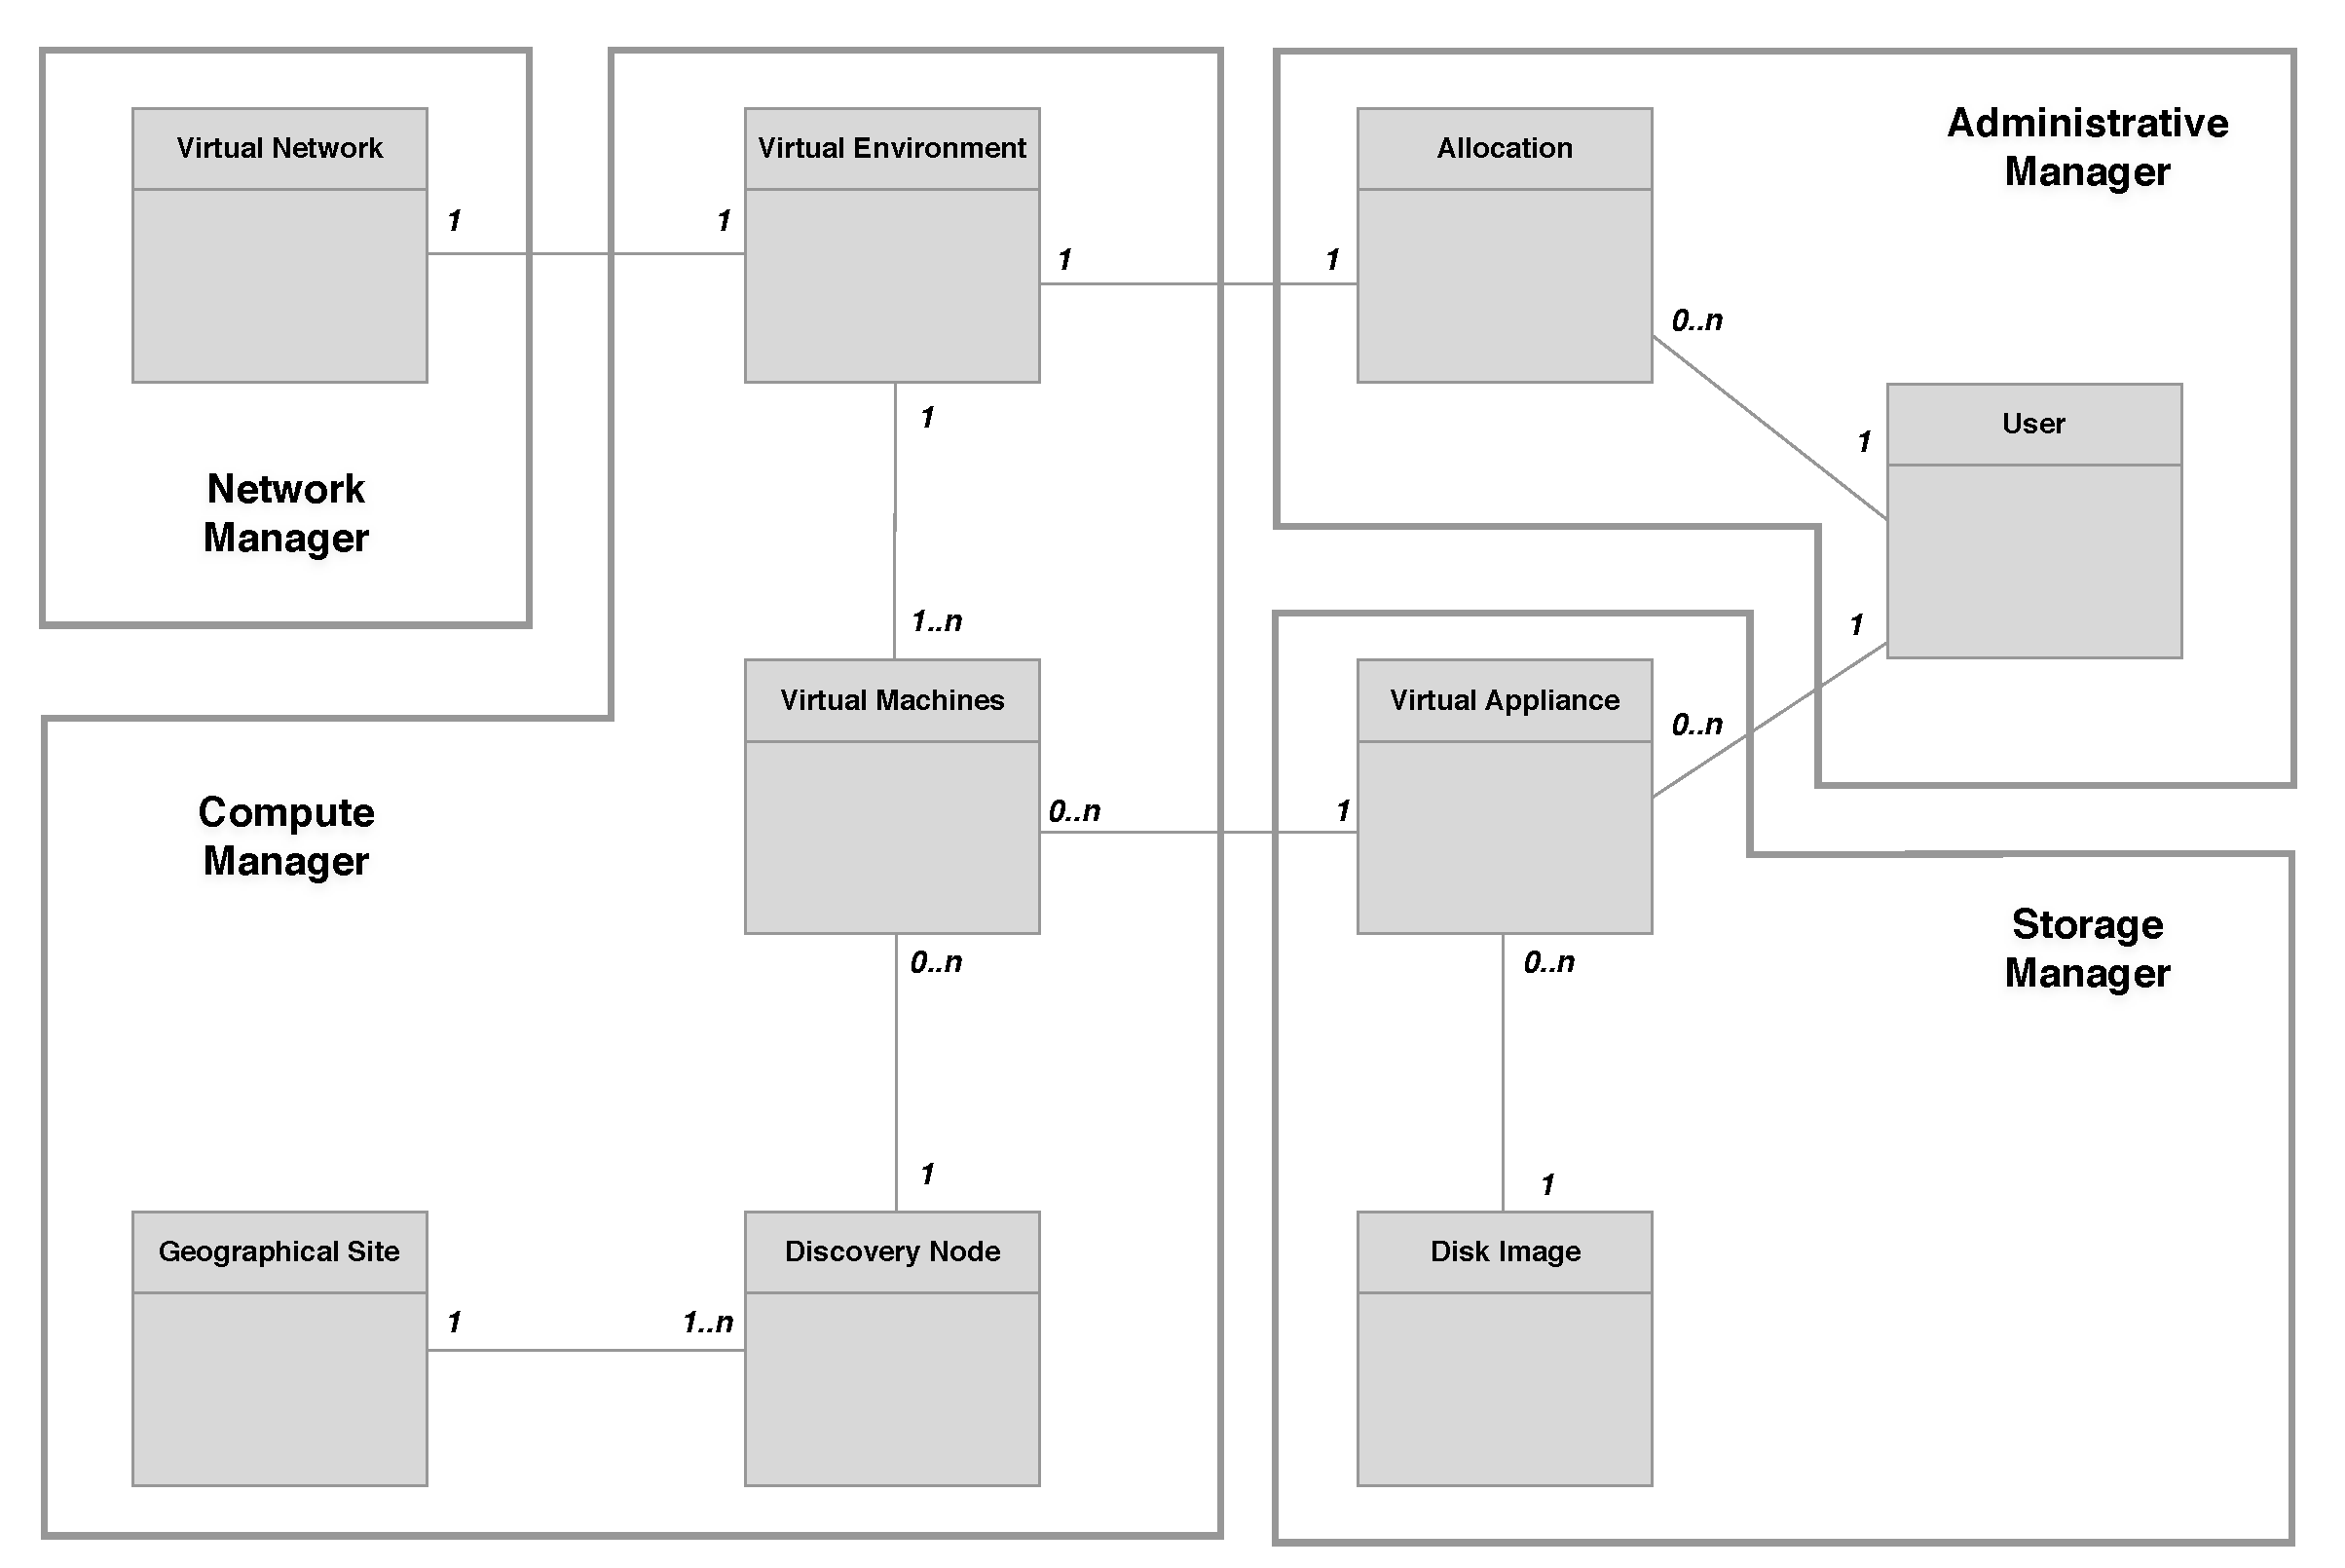
\includegraphics[width=0.91\linewidth]{Figures/mcd_3.pdf}
		\caption{Conceptual Data Model for Discovery proposal.}%
		\label{fig:mcd}%
		%\vspace*{-.8cm}
	\end{figure*}

	\item Virtual environment concept is the keystone of the Discovery proposal:
		
		\begin{itemize}

			\item When a user request the creation of virtual machines for a specified date, an allocation is registered.

			\item When the start date is reached, a virtual environment (isolated container for a VLAN and VMs) is created.

			\item a virtual environment can be run on several hosts, possibly spread over several geographical sites.

		\end{itemize}

	\item + description of other entities.

\end{itemize}

% \section{Revisiting existing cloud mechanisms}
\label{sec:integration}

\subsection{Openstack: a toolkit for building cloud}

\begin{itemize}
	
	\item Opensource project considered as a standard in cloud infrastrcutre.

	\item Composed of several "shared nothing architecture" services (nova, 
	swift, Quantum, Glance, ...).

	\item Uses an AMQP (Advanced Message Queuing Protocol) for inter-components 
	communication. => additional components can easily plug on an existing
	infrastructure.

	\item Drawack: Openstack does not perform dynamic scheduling of VMs.

\end{itemize}


\subsection{Revisiting components that are suitable for a LUC-OS (Related work)}

\begin{itemize}

	\item As we do not want to redevelop every services "from scratch", we will
	maximize the reuse of existing	mechanisms.

	\item In section \ref{sec:architecture} we defined a list of services provided 
	by the LUC-OS. Most of them will partially/completly leverage existing 
	mechanisms:

		\begin{description}

			\item [Compute manager] : 
			\begin{itemize}
				\item Nova is the service that is responsible for controlling 
				every services of the infrastucture. 

				\item It leverages nova-scheduler, which performs static 
				scheduling: nova-scheduler.

				\item We plan to use a dynamic scheduler (DVMS) instead.
			\end{itemize}

			\item [Administrative manager] : 
			\begin{itemize}
				\item KeyStone is the service used for managing identity and
				authentication.

				\item Horizon is the service that serves a web interface, 
				allowing users to interact with OpenStack.

				\item As we will use a distributed hash table (DHT) to save
				persistent states, we plan reuse Keystone and Horizon, with
				minor modification to leverage our DHT. 
			\end{itemize}

			\item [Storage manager] : 
			\begin{itemize}
				\item Swift is a distributed key/value service with no SPOF.
				
				\item Glance is a service for storing image that leverages 
				Swift. It is possible to directly store images in Swift.

				\item To limit network impact ("Boot problem"), solution based 
				on bittorrent have been developped (VMTorrent, 
				glance-bittorrent, ...).

				\item For a first prototype we propose to leverage Glance and
				Swift. If this solution become no more suitable for a massive
				infrastucture, we propose to integrate VMTorrent in Glance.

			\end{itemize}

			\item [Network manager] :
			\begin{itemize}
				
				\item Neutron is the service used to create VLAN.

				\item It supports plugins: it is possible to use Open vSwitch.
				This is what we propose for a first version of the system.

				\item For next versions, Mininet \ref{lanz:2010} or Vin can be
				considered as good candidates.
				
			\end{itemize}

		\end{description}

\end{itemize}



% 
%%%
\section{OpenStack for Operating Massively Distributed Clouds\label{sec:perspective_work}}

While advantages and opportunities of massively distributed clouds have been emphasized several years ago~\cite{church:2008, greenberg:2008},
delivering an OpenStack that can natively be extended to distinct sites will create new opportunities.
%Beyond the technical issues we should resolve to finalize our LUC OS, there are
%few challenges that our community should tackle to be able to fully use the
%technical capabilities offered by LUC infrastructures
We present in this section the most important ones and also raise associated challenges (beyond the technical issues we should resolve to finalize our
LUC OS) that our community should tackle to be able to fully use the technical capabilities offered by LUC infrastructures.

%% Beyond the technical issues we should resolve to finalize our LUC OS, a first important
%% challenge our community should shortly address to favor the adoption of such dynamic cloud
%% infrastructures is related to the automatic installation/upgrade of the LUC OS (\ie our
%% revised OpenStack software) throughout the different locations. In such a context,
%% scalability and geo-distribution make the installation/upgrade process more difficult as
%% it would probably require to relocate computations/data between locations in order to be
%% able to update physical servers without impacting the execution of hosted
%% applications. Another issue to investigate is whether it makes sense to extend a
%% deployment between several network operators and how such extensions can be handled. We
%% underline that even for such an extension (the term federation is probably more
%% appropriated in this situation), the two OpenStack systems will join each other to form a
%% single system. Of course security issues should also be addressed that are beyond the
%% scope of this paper. 

From the infrastructure point of view, a positive side-effect of our revised version of OpenStack is that it will natively allow the extension of a
private cloud deployment with remote physical resources. Such a scenario is a strong advantage in comparison to the current hybrid offers as it does
not break the notion of a single deployment operated by the same tenant. Each time a company will face a peak of activity, it will be possible to
provision dedicated servers and attach them to the initial deployment. Those servers can either be provided by dedicated hosting services that have
DCs close to the institution or by directly deploying transportable and containerized server rooms close to the private resources. This notion of
\emph{WANwide elasticity} can be generalized as it will be possible to deploy such containerized server rooms whenever and wherever they will be
mandatory. As examples, we can envision to temporarily deploy IT resources for sport events such as olympic games or for public safety purposes in
case of disasters. Network/Telecom operators will also be able to deploy IT resources on their radio base stations they operate in order to deliver
Fog/Edge computing solutions. The common thread in these use-cases is the possibility of extending an infrastructure wherever needed with additional
resources, the only constraint being to be able to plug the different locations with a backbone that offers enough bandwidth and quality of service to
satisfy network requirements. The major advantage is that such an extension is completely transparent for the administrators/users of the IaaS
solution because they continue to supervise/use the infrastructure as they are used to. The associated challenge our community should shortly address
to deliver such a \emph{Wanwide elasticity} is related to the automatic installation/upgrade of the LUC OS (\ie our revised OpenStack software)
throughout different locations. In such a context, scalability and geo-distribution make the installation/upgrade process more difficult as it
would probably require to relocate computations/data between locations in order to be able to update physical servers without impacting the execution
of hosted applications. Another issue to investigate is whether it makes sense to extend a deployment between several network operators and how such
extensions can be handled. We underline that even for such an extension (the term federation is probably more appropriated in this situation), the two
OpenStack systems will join each other to form a single system. Of course security issues should also be addressed, but they are beyond the scope of this
paper.

From the software point of view, developers will be able to design new applications but also revise major cloud services in order to deliver more
locality aware management of data, computation, and network resources. For instance, it will be possible to deploy on-demand Content Delivery Network
solutions according to specific requirements. Cloud storage services could be revised to mitigate the overheads of transferring data from sources to
the different locations where there are needed. New strategies can favor for instance a pulling mode instead of a pushing one. Nowadays data is
mostly uploaded to the remote clouds without considering whether such data movements are effectively solicited or not. We expect that LUC
infrastructures will enable data to stay as close as possible to the source that generates them and be transferred on the other side only when it will
be solicited. Such strategies will mitigate the cost of transferring data in all social networks for instance. Similarly, developers will be able to
deliver Hadoop-like strategies where computations are launched close to data sources. Such mechanisms will be shortly mandatory to handle the huge
amount of data that Internet of Things will generate. However, delivering the LUC OS will not be sufficient to allow developers to implement such new
services. Our community should start as soon as possible to revise and extend current interfaces (\aka Application Programming Interfaces). In
particular, the new abstractions should allow applications to deal with geo-distribution opportunities and contextual information by using them to
specify deployment/reconfigurations constraints or to develop advanced adaptation scenarios in order to satisfy for instance SLAs.

Finally, the last opportunity we envision is related to the use of renewable energies to partially power each PoP of a LUC infrastructure. Similarly
to follow-the-moon/follow-the sun approach, the use of several sites spread across a large territory will offer opportunities to optimize the use of
distinct energy sources (solar panels, wind turbines). While such an opportunity has been already underlined~\cite{Berral:2014:BGC:2672596.2672694},
the main advantage is once again related to the native capability of our revised OpenStack to federate distinct sites, allowing users to use such a
widely distributed infrastructure in a transparent way while enabling administrators to balance resources in order to benefit from green energy
sources when available (since the system is supervised by a single system we expect that the development of advanced load-balancing strategies
throughout the different servers composing the infrastructure would be simplified).

%%  + Quels sont les challenges/opportunités d'un cloud massivement distribué (SWOT)
%%    - Strengths
%%      + locality aware management of data, computation and network resources
%%      + fault-tolerance (leveraging geo-distributed locations)
%% + Scalability (additional resources can be added to the infrastructure whereever it is, the only constraint is to be able to plug those resources to the LUC infrastructure
%%    - Weaknesses: 
%%  - resource management complexity from the administrator viewpoint (no single view of the whole platform, maintenance of the hardware) 
%%  => Contre balancer avec l'aspect fiabilité dans les forces
%%       - Mutualization of resources is questionable and should be better investigated (economical/energy, on-going work) 
%%       - security (in terms of Human presence) of micro DCs.
%%       - network peering agreement (how can we extend a LUC infrastructure beyond one operator). 
%%    - Opportunites: 
%%      + Revise major cloud services to take benefit from the massively distributed clouds
%%        - Cloud storage locality aware services
%%        - CDN on demand (with particular topology) 
%%     + Create new (and smarter) services (that needs computations capabilities closer to end-users) such as 
%%       - public safety, deploy IT on demand and where it is mandatory and plug it to the whole infrastructure. 
%%       - IOT  
%%          + big computations can be performed as close as possible to the sensors)
%%          + Use of sensors to create new services (smart cities)
%%          +  Mobile computation and data management, cloudlet (i.e. virtual representation of the physical devices follows the localtion of the device, the cloudlet can benefit from the power of the LUC infrastructure while following the device)  
%%          + Advanced data processing enabling the mitigation of data transfer (avoiding the movement of large and useless data items)
%%         + Digital heater farm (Qarnot Computing / Aoterra) - http://www.qarnot-computing.com/technology  / https://www.cloudandheat.com/en/index.html
%%     + Use of renewable energy (follow the moon, follow the sun, follow the wind, ...) 
%%   - Threats: 
%%      + Accouting, billing and monitoring 
%%      + Ensure QoS
%%      + Mise à jour de l'infrastructure (modificiation des couches logicielles à chaud
%%     + Security of communications at every level of the stack. 


\section{Reference architecture for IaaS clouds}

Recent studies have showed that state of the art IaaS manager \cite{peng:2009}
were constructed over the same concepts. Furthermore a reference architecture 
for IaaS manager has been described in \cite{moreno2012iaas} enabling the design
of an IaaS toolkit. Besides the reference architecture, an IaaS toolkit should
provides some mechanisms that enables to solve the scalability problem.

In a recent study, authors have proposed a reference architecture for 
a Cloud OS \cite{moreno2012iaas}: they aimed at providing abstractions of 
underlying technologies that compose current IaaS managers. The strength of 
their work resides in the fact that they considered all the needs of an 
"industrial class" IaaS manager: each of its functions has been widely studied.
Beacause we find this work well detailed, we have decided that a new 
architectural proposition for a distributed IaaS manager should leverage this 
work.

\section{Designing the LUC-OS}
\label{sec:lucos}


% - Section 2: presentation of a reference architecture with challenges 
%   overview.
% - generic architecture -> can be applied to centralized, partially
%   distributed (federation of clouds) and fully distributed (LUC-OS) Cloud OS.
% - LUC-OS design is different of a classical IaaS manager (Controller ->
%   distributed share no state algorithm, DataBase -> DHT, Distributed FS -> p2p
%   FS), this section will expose the development methodology.
Section \ref{sec:moreno} exposed a reference architecture for building a Cloud 
OS, which have been proposed by \cite{moreno2012iaas}: this architecture is 
generic in the sense that it provides a model where each aspect of the Cloud OS 
is managed by a dedicated service. As a consequence, this model can be used as 
well for centralized clouds, partially distributed clouds (federations of 
clouds) and fully distributed clouds. The LUC-OS targets a fully distributed 
functioning, which is not the principal aim of current open-source Cloud 
managers, and thus requires a significantly different architecture oriented 
towards the management of massively distributed clouds.

% - Distributed clouds : hundreds micro DCs, which are themselves composed of up
%   to tens of servers 
% - Managing a distributed cloud -> managing thousands of geographically spread 
%   hosts.
% - P2P file sharing systems: example of software that works well in similar
%   conditions.
% - We think the file sharing systems should be an inspiration for the LUC-OS
%   design.
A massively distributed cloud is an infrastructure that is composed of up to 
hundreds of micro DCs, which are themselves composed of up to tens of servers, 
thus operating such infrastructure means managing up to thousands of
geographically spread servers. Designing software that works at this scale is a
tedious task, as it comes with challenges such as preserving a good reactivity 
and implementing working fault tolerance mechanisms. Peer to peer file sharing 
systems (popular over the last decade) are a good example of software that works
well at large scale in a context where computing resources are geographically 
spread. That is why we propose to learn from the experience of large scale peer 
to peer systems : design rules of the LUC-OS architecture will be directly 
inspired by them. 

\subsection{Design rules}

% - LUC-OS: distributed system: workload divided among every peers.
% - LUC-OS is a multi-agent system: each server (node) of the infrastructure 
%   host one LUC-OS agent.
% - A LUC-OS agent is composed of several services, each service is specialized
%   in a particular task.
% - To prevent bottlenecks and single point of failure, each service is 
%   distributed in a fully distributed manner: 
%    * bottleneck: in case a service is overloaded, it must be able to balance
%      workload on remote service instance.
%    * single point of failure: at large scale, failure becomes the norm rather
%      than the exception, services must implement self healing mechanisms and
%      each persistent state is stored in fault tolerant data structure (DHT).
% - To maximize the reactivity of the LUC-OS, a service should prioritize 
%   collaboration with corresponding services hosted on servers accessible with
%   low latency.
% - To enable low-latency collaborations, each service will leverage a locality
%   based overlay that will dynamically maintain for each server a list of 
%   neighbors.
The LUC-OS targets a fully distributed functioning inspired by the peer to peer
paradigm : its workload will be allocated over among every element constituting
the infrastructure. As we are interested by adding advanced properties 
(self-organization and self-healing) to the LUC-OS, we propose to leverage a 
multi-agent architecture: each node (server) constituting the infrastructure 
will host one of the LUC-OS agent. To prevent negative phenomenons such as
bottlenecks and single points of failure (SPOF), we have decided to anticipate
them during the design stage:

\begin{description}

  \item [Bottlenecks] : are caused by an excessive workload allocated to one 
  service, which slows its interactions with collaborators, thus impacting
  negatively the performance of the infrastructure by reducing both reactivity 
  and quality of service. Indeed, when a service is overloaded, it is better to 
  enable him to distribute the workload on several remote instances that are
  underloaded.

  \item [Single points of failure] (SPOF) represents an element of a system, 
  that in case of failure, stops the entire system. As at large scale, failure 
  becomes the norm rather than the exception, SPOFs are a major concern in
  distributed software: that is why services must implement self healing 
  mechanisms such as redundancy. In addition each persistent state have to be 
  stored in fault tolerant data structure like a distributed hash-table (DHT).

\end{description}

\subsection{Anatomy of a LUC-OS agent}


\begin{figure*}
	\centerline{
	 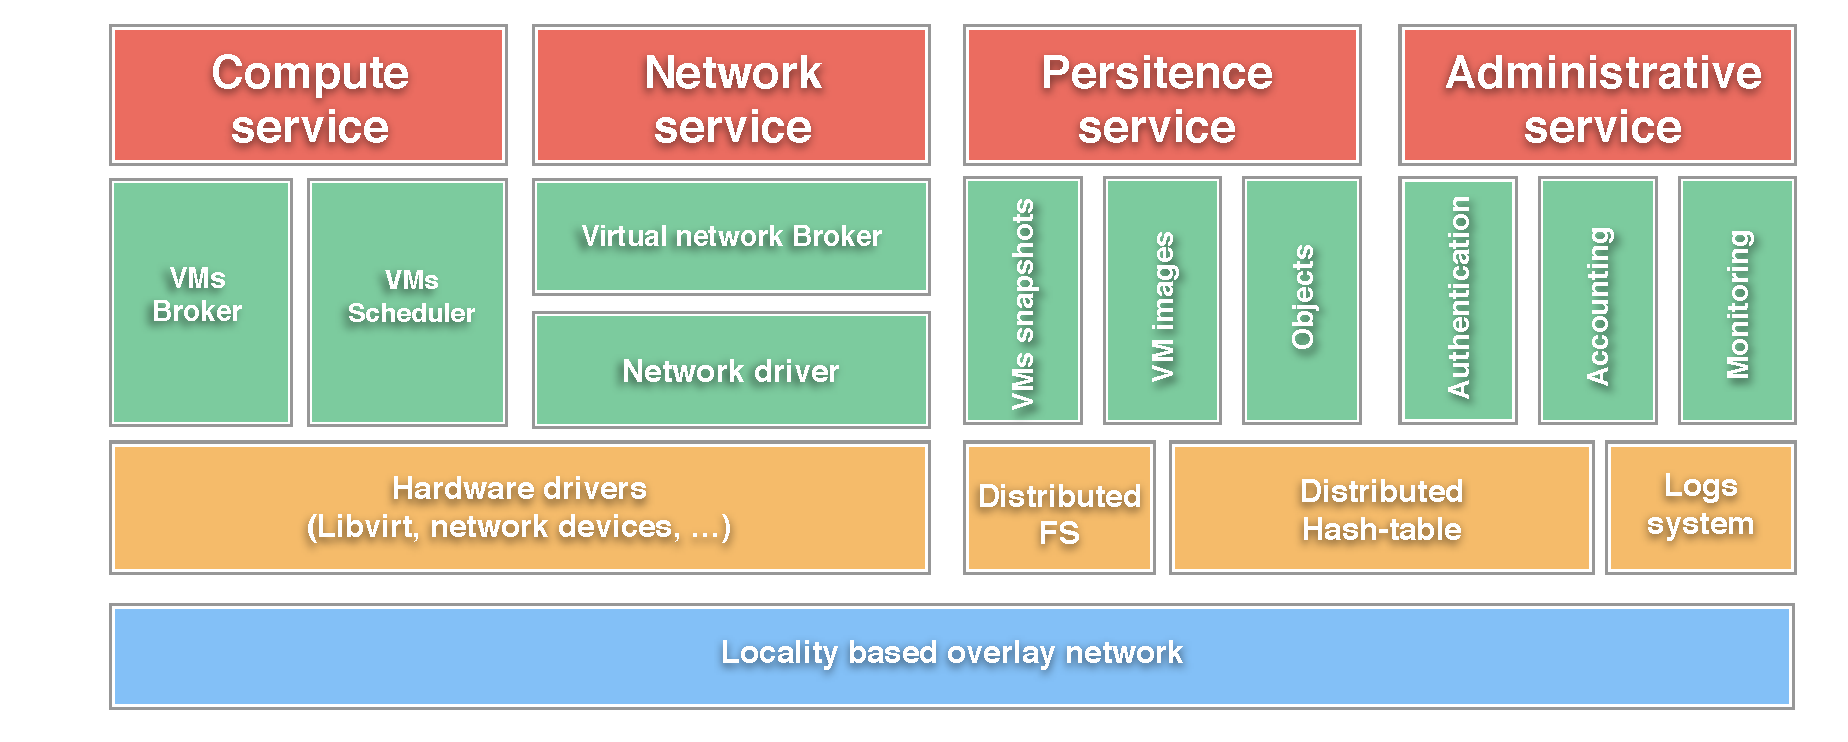
\includegraphics[width=1.25\linewidth]{Figures/luc_os_anatomy.pdf}
  }
	\caption{Anatomy of services composing the LUC-OS.}%
	\label{fig:anatomy}%
	%\vspace*{-.8cm}
\end{figure*}

% - Figure \ref{fig:anatomy} -> our choices
% - 4 services: one service per aspect (compute, network, persistance, admin). 
% - Compute service: delivery of computing resources: built on top of:
%    * VMs broker: receives VM creation request, elect a server: it instantiate 
%      the VM; ensures VM creation.
%    * VMs scheduler: ensures good QoS for VMs: compute node overloaded ->
%      sched balances workload on underloaded ones (dynamic scheduling).
% - Network service: create virtual that interconnect VMs (broker). Network 
%   creation abstracted by the use network drivers (OpenFlow, Mininet, ...).
% - As some services manipulate hardware -> direct access via Hardware Drivers.
% - Persistence service: store states manipulated by the services of the LUC-OS:
%    * Objects (serializable entities); VMs images (VMs template) belonging to a 
%      specific user (+ metadata); VMs snapshots: like VM images with versions.
% - These sub-services leverage a DHT, and some of theme leverage a resilient 
%   distributed FS.
% - Administrative: managing the infrastructure and producing statistical and 
%   usage data.
% - To perform those tasks it will leverage a DHT and a service that store 
%   execution logs of the infrastructure.

\label{sec:anatomy_lucos}
Figure \ref{fig:anatomy} depicts our architectural choices: each aspect of the 
LUC-OS is managed by a specific service that will collaborate with close 
instances of the service located on remote nodes through the use of locality
based network overlay. 

\subsubsection{Compute service}
is in charge of the delivery of computing power: it is built on top of two 
sub-services : \emph{VMs broker} which process requests for VMs creation (static
scheduling: it elects a server that will instantiate the VM and ensures that the
VM is successfully created) and \emph{VMs scheduler} that guarantees a good 
quality of service for VMS by balancing workload of overloaded compute node on
underloaded ones (dynamic scheduling). 

\subsubsection{Network service} 
leverages a \emph{virtual network Broker} that create virtual networks 
interconnecting VMs. Creation of these virtual networks is abstracted by the use
of \emph{Networking drivers}: it enables the use of a wide range of network 
technology such as OpenFlow and Mininet. As all services composing Compute 
service and network drivers manipulate hardware, they will have direct access to
hardware via Hardware Drivers. 

\subsubsection{Persistence service}
is dedicated to keeping states of the LUC-OS by leveraging one service for each
kind of state: \emph{Objects} are used to persist serializable entities 
manipulated by the LUC-OS, \emph{VMs images} are used for VMs template files 
(which belong to a specific user), \emph{VMs snapshots} are pretty much the same
as VM images except that they support versionning. All the sub-services that 
compose the Persistence service leverage a distributed hash-table, and those 
which are in charge of persisting images and snapshots will leverage a resilient 
distributed file system. 

\subsubsection{Administrative service} 
will perform tasks such as managing the infrastructure and producing statistical
and usage data. To perform those tasks it will leverage a distributed hash table
and a service that stores execution logs of the infrastructure.





\section{Revising OpenStack}
\label{sec:leveraging-openstack}

OpenStack is an open-source project that aims at developing a complete cloud management
system. Similary to the reference architecture described in the previous Section, it is
composed of several services, each one dealing with a particular
aspect of a Cloud infrastructure as depicted in Figure~\ref{fig:openstack}.

\begin{figure}[htbp]
        \centering
        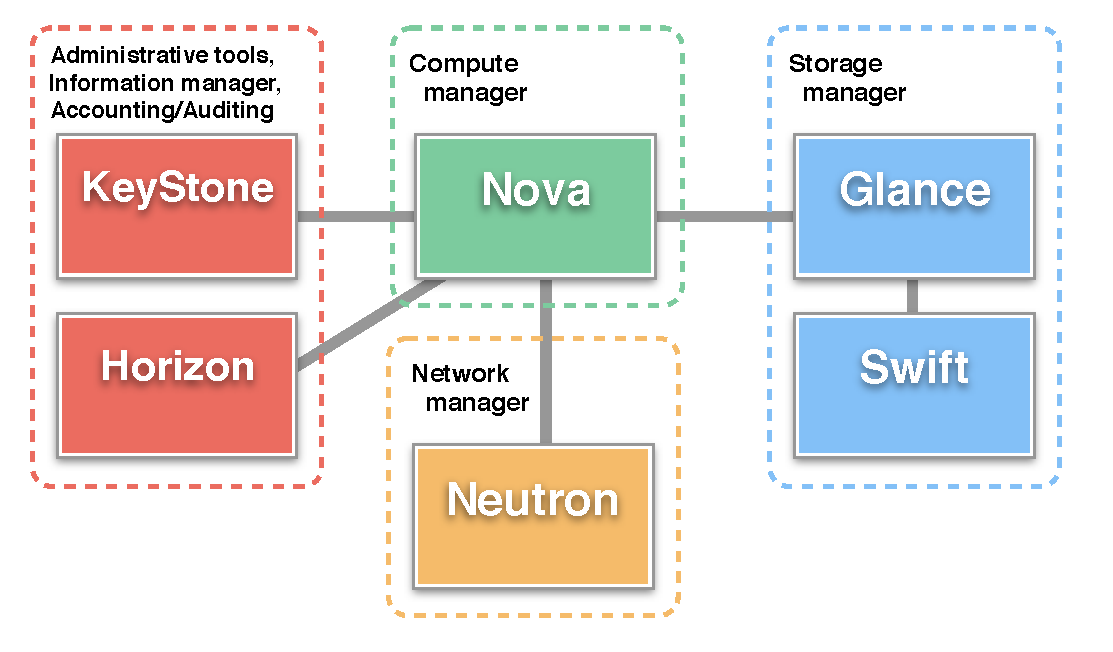
\includegraphics[width=6cm]{figures/OpenStack_architecture.pdf}
\vspace*{-.3cm}
        \caption{Services composing OpenStack.}
        \label{fig:openstack}
\vspace*{-.3cm}
\end{figure}


OpenStack relies on two kinds
of nodes: controller and compute node. The former is in charge of managing and
distributing work to the latter that provides computing/storage resources to end-users. In
other words, the controllers correspond to the different services introduced in the
previous section while the compute nodes host the VMs.

From the software point of view, the OpenStack architecture is based on the ``shared
nothing" principles: each controller (\ie each service) is connected to the others via two
different way:

\begin{itemize}
   \setlength{\itemsep}{0pt}
  \setlength{\parskip}{0pt}
   \setlength{\parsep}{0pt}
\item \textbf{A messaging queue} that enables the collaboration between sub-services of a
  controller.
\item \textbf{A SQL database} (DB) that stores inner states of a controller.
\end{itemize}

Finally, the controllers interact with each other through REST APIs or directly by accessing
the inner-state that are stored in the differents DBs.
%\AL[JP]{Is it correct ? How the controllers interaact/collabore ?}

Considering the current structure of OpenStack, the main limitation to make it distributed
is related to the SQL databases. Indeed, while OpenStack relies on the
RabbitMQ messaging service, which is articulated around a centralized
broker, there are few implementations of  P2P messaging
service such as ActiveMQ~\cite{activemq:2011} or ZeroMQ~\cite{zeromq:2013} that would be adapted to the LUC requirements.
% \section{Towards a fully distributed OpenStack deployment}
%
% The discovery initiative targets the delivery of an utility computing platform
% that will be working on top of existing network backbone facilities. Starting
% the development of such a platform from zero would require a titanic effort: in
% order to spare a giant development time, the Discovery initiative proposes to
% leverage the OpenStack project: this will serve as the foundation of the
% LUC-OS.
%
% In order to structure the LUC-OS on a fully distributed peer to peer
% functionning, OpenStack would be required to be fault tolerant and to be able to
% fit on a multi-site configuration. In the current situation, it requires some
% adaptations: in this section we propose some modifications that
% have been introduced in the Nova controller, to meet the two
% aforementioned criterions.
%
% \subsection{Replacing the relational backend by a Key/value store}
%
% From today's perspective, most of the OpenStack deployment are involving few
% nodes, thus not requiring more thant one controller. However, to meet the fault
% tolerance criterion, one needs to use \textit{High availibility} deployment by
% combining two components \textit{HAProxy} (load balancing) with
% \textit{Galera} (Relational database replication).
The first way to bypass the MySQL limitation is to
% a controller between distinct locations,
%\ie to be able to scale in/out the services it offers, is to
deploy each controller DB on each location and to synchronize the different DB
instances with a dedicated mechanism~\cite{kemme:vldb2010}. By such a mean, when a
controller processes a request and performs some actions on one site, changes in the
inner-state are also propagated to all the other locations. From a certain point of view,
it gives the illusion that there is only one DB for each service. Although the technique
described has been used in different proof-of-concepts, current DB synchronization
mechanisms are not scalable enough to cope with a LUC infrastructure deployed on large
number of geographical sites.

Another approach is to replace the DBs used in OpenStack by a more suitable storage
backend that would provide a better scalability. Distributed Hash Tables (DHTs) and more
recently key/value systems built on top of the DHT concept such as
\emph{Dynamo}~\cite{decandia:dynamo} have demonstrated their efficiency in terms of
scalability and fault tolerance properties.
%
In light of this, we have revisited the Nova controller, \ie the VM manager of OpenStack,
in order to to replace the current MySQL DB system by \textit{REDIS} ~\cite{han:2011},
a \textit{key/value store}.
% that extends the principles followed by the \textit{Dynamo}. %with more advanced storage and query features.
Technically speaking, we modified the Nova database driver. Indeed, the  Nova software architecture has been
organised in a way which ensures that each of its sub-services does not directly manipulate the database: they have an indirect
access through a service called ``nova-conductor" which in turn works with an
implementation of the \textbf{"nova.db.api"} programming interface. Developers of Nova
provide an implementation of this interface that is using \textit{SQLAlchemy} to
manipulate a relational database. We developed a second implementation of this interface
that replaces every call to the \textit{SQLAlchemy} by a call to a
custom key/value store
driver.  This enables  Nova's services to work with REDIS by only changing the
database driver, limiting the level of intrusiveness in the original source code.
Thanks to this modification, it is possible to instanciate  a distributed
cloud and operate it through a single instance of OpenStack composed
of several Nova controllers deployed on distinct sites.
Figure~\ref{fig:newnova} depictes such a deployment.
%
Each controller executes a REDIS instance that is configured to work in
a clustering way with other instances.
One or several controllers can be deployed on each site according to
the expected demand in terms of end-users. Finally, a controller can be
deployed either on a dedicated node or be mutalized with a compute
one as illustrated for Site 3. We higlight that any controller can
provision VMs by orchestrating services on the whole infrastructure and not only on the site
where it is deployed. Such a behavior is possible thanks to the AMQP
bus and the key/value store that go through all controllers.
%
Finally, it is noteworthy that key/value stores that
focus on high-availability and partition tolerance criteria like
Cassandra~\cite{lakshman:2010} would be more appropriate than REDIS
for a production deployment. We chose REDIS for its usage simplicity.

\begin{figure}[htbp]
        \centering
\vspace*{-.4cm}        \hspace*{-.2cm}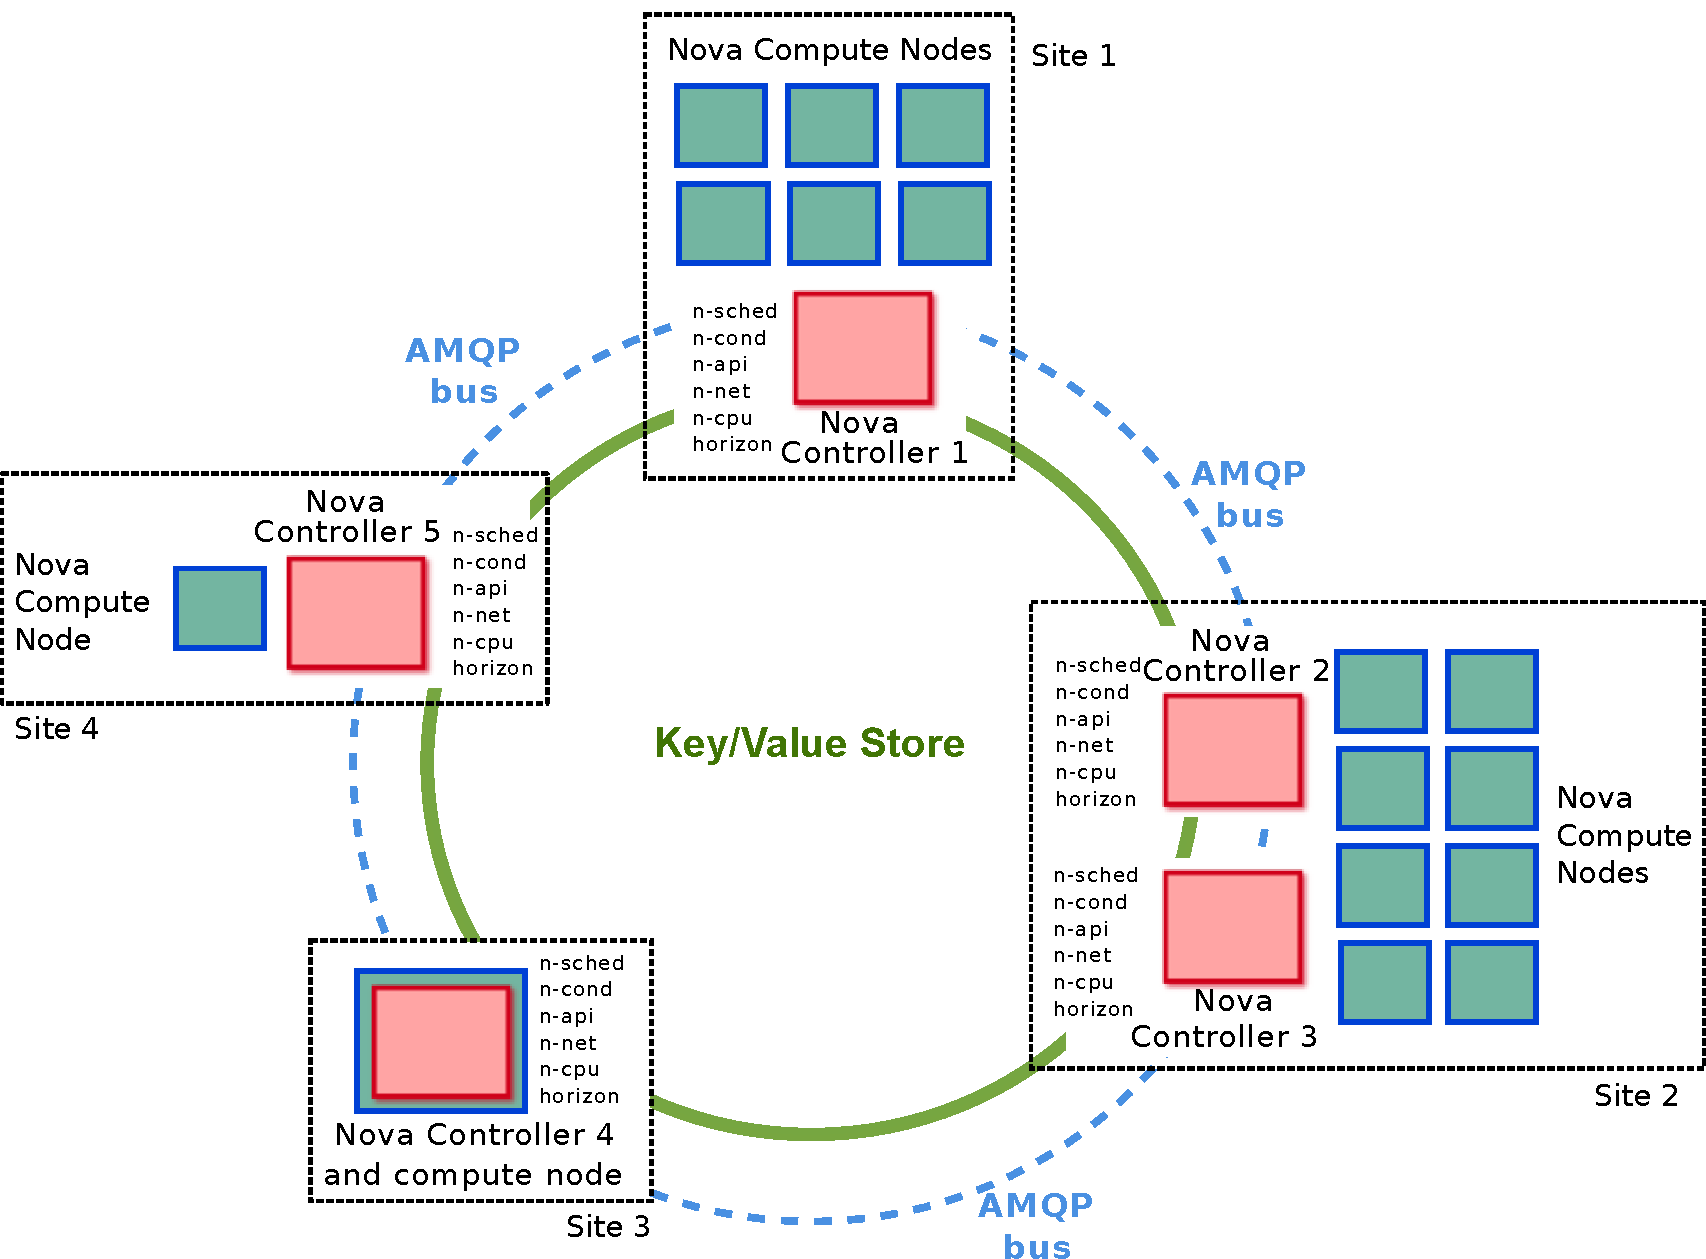
\includegraphics[width=.51\textwidth]{figures/OpenStack_distributed.pdf}
        \caption{Nova controllers are connected through a shared key/value backend
        and the AMQP bus.}
      \label{fig:newnova}
\vspace*{-.3cm}
\end{figure}

Our prototype is under evaluation.
However, preliminary experiments  have been performed throughout 4
sites of Grid'5000  including 12 compute nodes  and 4 controllers
overall. While this
infrastructure was rather small in comparison to our target, it aimed
at validating the interconnection of several controllers WANwide and
the correct behaviour of  OpenStack using our noSQL backend.
Our prototype suceeded to provision 500 VMs in 300 seconds
(each controller creating 125 VMs in parallel).
A second experiment validated the provisionning
of 2000 VMs in less than 30 min.  We are currently performing comparisons
between OpenStack using the historical MYSQL backend \textit{v.s.,}
using a key/value store backend. Our goal is to validate that
manipulating internal states of Openstack through
a noSQL deliver performances in the same order of the MySQL
ones.



Cloud Computing has entered our everyday life at a very high speed and huge scale. From classic high performance computing simulations to the management of huge amounts of data coming from mobile devices and sensors, its impact can no longer be minimized. While a lot of progress has already been made in Cloud technologies, there are several concerns that limit the complete adoption of the Cloud Computing paradigm.

In a previous report~\cite{lebre:hal-00854204}, we outlined that, in addition to these concerns, the current model of UC is limited by intrinsic issues. Instead of following the current trend by trying to cope with existing platforms and network interfaces, we proposed to take a different direction by promoting the design of a system that will be efficient and sustainable at the same time, putting knowledge and intelligence directly into the network backbone itself. The innovative approach we introduced will definitely tackle and go beyond Cloud Computing limitations. Our objective is to pave the way for a new generation of Utility Computing that better matches the Internet structure by means of advanced operating mechanisms. By offering the possibility to tightly couple UC servers and network backbones throughout distinct sites and operate them remotely, the LUC OS technology may lead to major changes in the design of UC infrastructures as well as in their environmental impact. The internal mechanisms of the LUC OS should be topology dependent and resources efficient. The natural distribution of the nodes through the different points of presence should be an advantage, which allows to process a request according to its scale: Local requests should be computed locally, while large computations should benefit from a large number of nodes.

The first step toward this highly distributed Cloud infrastructure taking into account locality and network distance is the scheduling of VMs taking into account locality. Thus is this paper, we presented our first building block of our distributed Cloud infrastructure that consists in using P2P algorithms and a vivaldi overlay connected to DVMS, an efficient and flexible VMs scheduler. Our first experiments over Grid'5000 show that, connecting 4 differents sites and scheduling VMs over them, we can gain up to 66\% of inter-sites operations. 

Our future work will consist in ... 


\bibliographystyle{abbrv}
\bibliography{main}

\end{document}
